\chapter{Wyniki}

Po stworzeniu aplikacji przeprowadzone zostały testy mające na celu sprawdzić wydajność aplikacji pod kątem czasu wykonania oraz porównanie wyników, wykonując te same obliczenia korzystając jedynie z mocy CPU. 
Poniżej zamieszczone zostały wyniki tych pomiarów.

\begin{figure}[h]
\centering
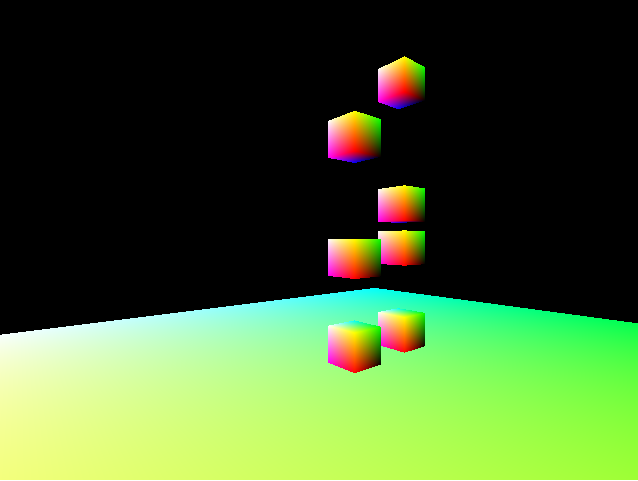
\includegraphics[width=0.4\textwidth]{figures/app1.png}
\caption{Przykładowy zrzut ekranu z aplikacji (opracowanie własne).}%
\label{rys:Przykladowy zrzut ekranu z aplikacji}
\end{figure}
\begin{figure}[h]
\centering
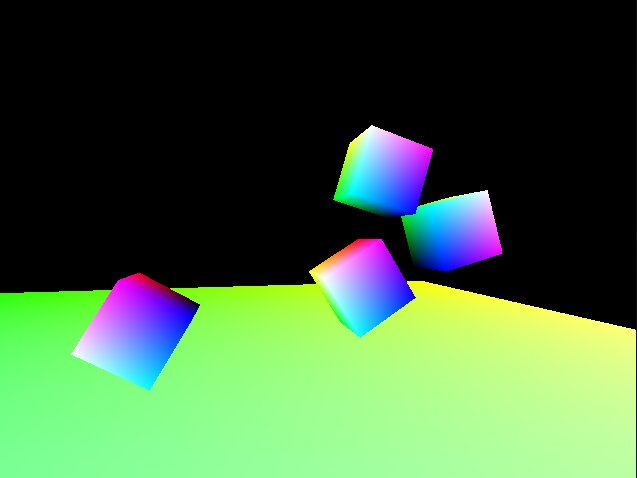
\includegraphics[width=0.4\textwidth]{figures/app2.png}
\caption{Zrzut ekranu z aplikacji po kolizji (opracowanie własne).}%
\label{rys:Zrzut ekranu z aplikacji po kolizji}
\end{figure}
\begin{figure}[h]
\centering
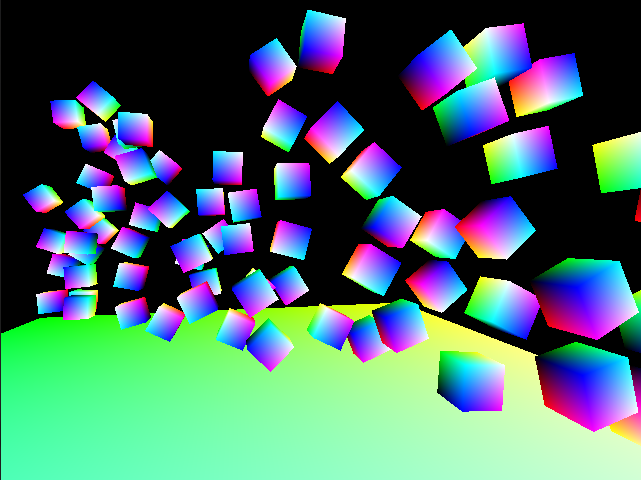
\includegraphics[width=0.5\textwidth]{figures/app3.png}
\caption{Zrzut ekranu z aplikacji po kolizji (opracowanie własne).}%
\label{rys:Zrzut ekranu z aplikacji po kolizji}
\end{figure}
\begin{tabular}{|c|c|c|}
\hline
Liczba brył & Czas wykonania GPU (ms) & Czas wykonania CPU(ms) \\
\hline
1 & 46.3 & 16.7\\
2 & 46.3 & 16.7\\
5 & 46.3 & 16.7\\
10 & 46.3 & 16.7\\
100 & 52.4 & 167.8\\
1000 & 90.6 & ponad 1000\\
\hline
\end{tabular}
\newline
\newline
\newline
Tabela przestawia uśrednioną wartość czasu potrzebną na wykonanie jednej iteracji zawierającej aktualizację pozycji obiektów oraz wyznaczanie kolizji i obliczanie wartości sił po zderzeniu. Każdy przedstawiony wynik to średnia arytmetyczna z 1000 pomiarów. Można zauważyć, iż czas potrzebny na wykonanie tych operacji w zakresie do 10 brył w symulacji jest niezmienny. Jednocześnie widać, że do tego momentu wykonywanie operacji na CPU przynosi większe korzyści, niż na GPU. Zdarzenie to spowodowane jest dodatkowym czasem potrzebnym na utworzenie buforów oraz przesyłanie ich do oraz z urządzenia GPU. Natomiast wraz ze wzrostem liczby symulowanych obiektów średni czas operacji zwięsza się zdecydowanie szybciej dla testu przeprowadzonego na CPU. Dzięki możliwości równoległego wykonywania operacji na wielu obiektach jednocześnie, czas potrzebny na wykonanie operacj rośnie zdecydowanie wolniej niż ma to miejsce przy wykorzystaniu CPU.\\